\documentclass[problem]{mcs}

\begin{pcomments}
  \pcomment{MQ_expectHH_TT}
  \pcomment{similar to MQ_expectHHH}
  \pcomment{shorter variation of CP_consecutive_coin_flips}
  \pcomment{ARM 5/6/12}
\end{pcomments}

\pkeywords{
  expectation
  total_expectation
  probability_tree
  tree_model
}

%%%%%%%%%%%%%%%%%%%%%%%%%%%%%%%%%%%%%%%%%%%%%%%%%%%%%%%%%%%%%%%%%%%%%
% Problem starts here
%%%%%%%%%%%%%%%%%%%%%%%%%%%%%%%%%%%%%%%%%%%%%%%%%%%%%%%%%%%%%%%%%%%%%

\begin{problem}
  A coin with probability $p$ of flipping Heads and probability $q \eqdef
  1-p$ of flipping tails is repeatedly flipped until two consecutive flips
  match---that is, until HH or TT occurs.  The outcome tree $A$ for
  this setup is illustrated in Figure~\ref{HH-TT-tree}.

    \begin{figure}
      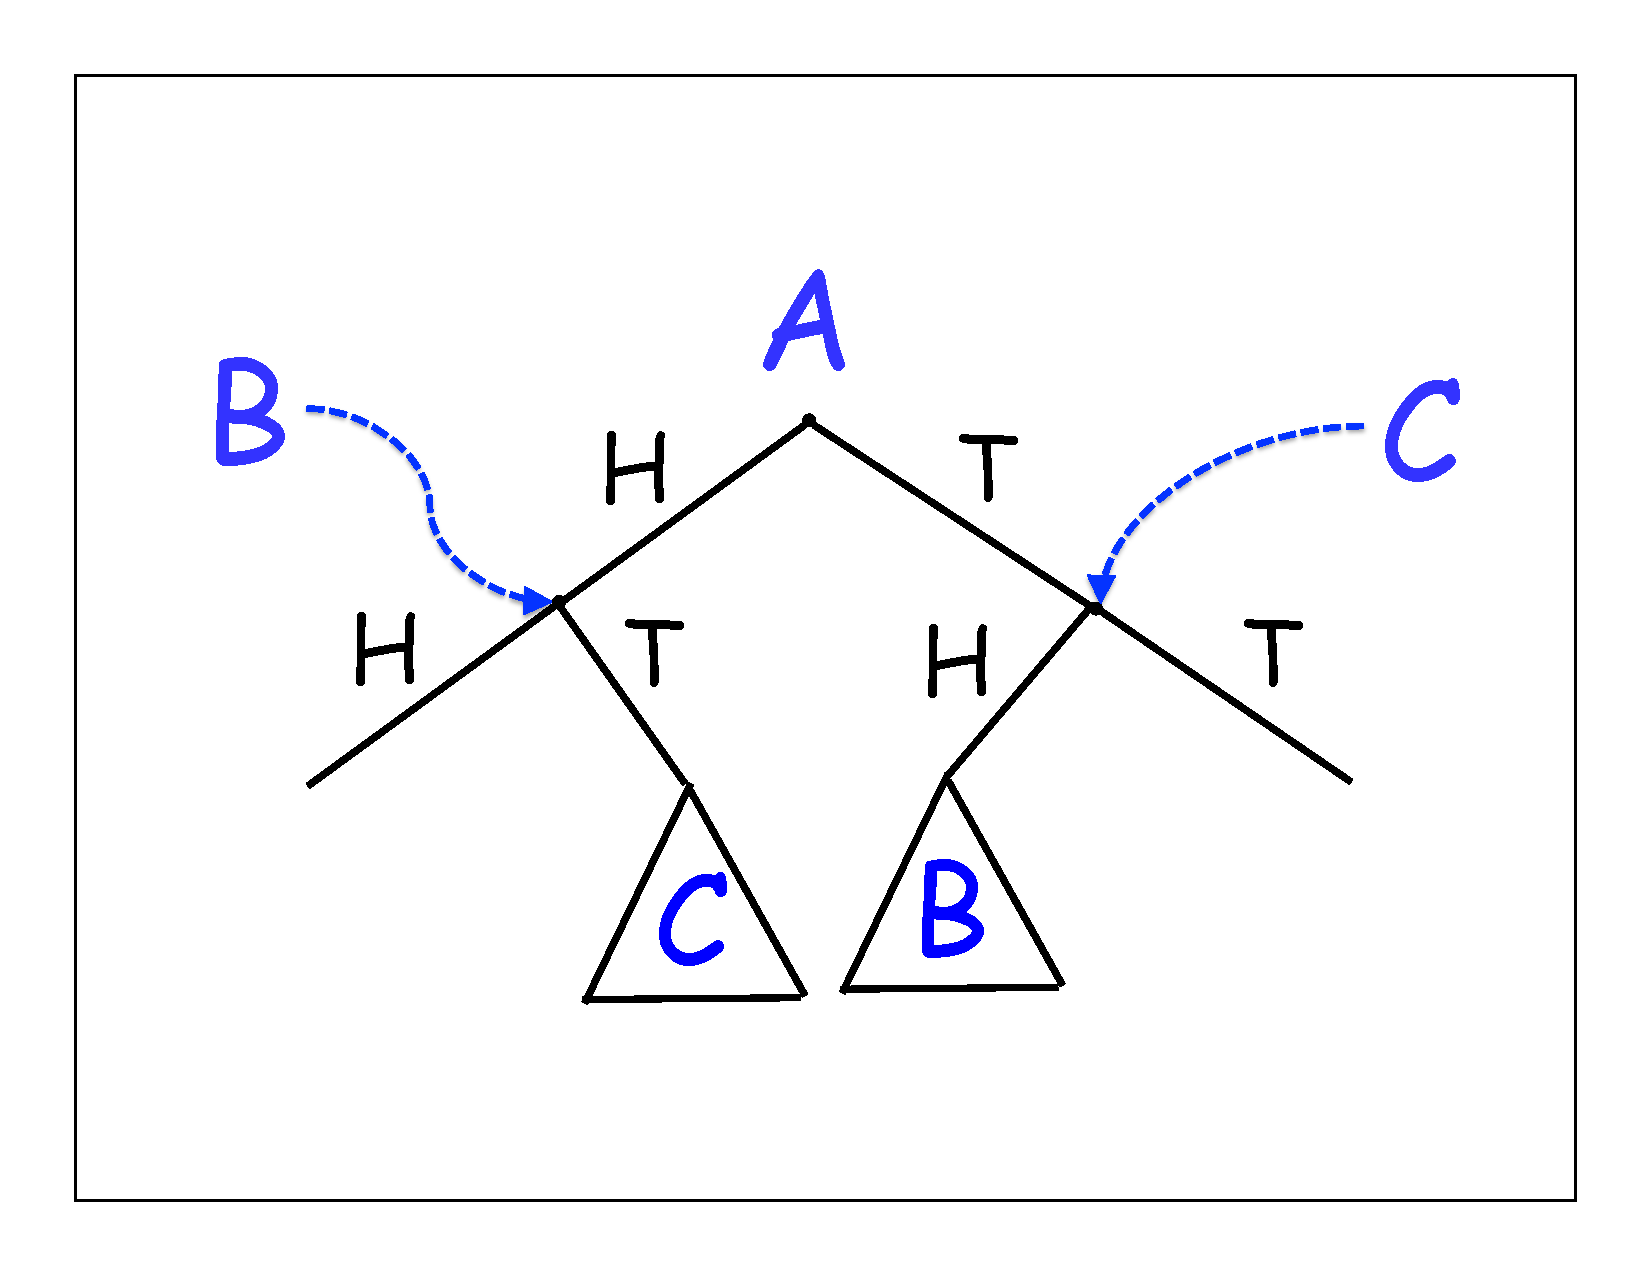
\includegraphics[width=3.5in]{HH-TT-tree-frame}
     \caption{Outcome Tree for Flipping Until HH or TT}
     \label{HH-TT-tree}
    \end{figure}

Let $e(T)$ be the expected number of flips starting at the root of
subtree $T$ of $A$.  So we're interested in finding $e(A)$.

Write a small system of equations involving $e(A), e(B)$, and $e(C)$
that could be solved to find $e(A)$.  \emph{You do \textbf{not} need
  to solve the equations.}

\begin{solution}
By the Total Expectation Rule, we have
\begin{align*}
e(A) & = p(1+ e(B)) + q(1+e(A)) = 1 + pe(B) + qe(C),\\
e(B) & = p(1+ e(C)) + q(1+0)    = 1 + pe(C),\\
e(C) & = p(1+ 0) + q(1+e(B))    = 1 + qe(B).
\end{align*}

A solution to these equations was not called for, but is easy to work
out.  Namely, substituting for $e(C)$, we get
\[
e(B) = 1 + p + pqe(B),
\]
so
\[
e(B) = \frac{1+p}{1-pq}\ .
\]
Similarly,
\[
e(C) = \frac{1+q}{1-pq}\ .
\]
Therefore,
\begin{align*}
e(A) & = 1 + \frac{p(1+p)}{1-pq} + \frac{q(1+q)}{1-pq}\\
     & = 1 + \frac{p(1+p)+ q(1+q)}{1-pq}\\
     & = 1+ \frac{p+p^2+ 1-p +1-2p+ p^2)}{1-p+p^2}\\
     & = 1+ \frac{2-2p+ 2p^2)}{1-p+p^2}\\
     & = 1+2 = 3.
\end{align*}

\end{solution}

\end{problem}


%%%%%%%%%%%%%%%%%%%%%%%%%%%%%%%%%%%%%%%%%%%%%%%%%%%%%%%%%%%%%%%%%%%%%
% Problem ends here
%%%%%%%%%%%%%%%%%%%%%%%%%%%%%%%%%%%%%%%%%%%%%%%%%%%%%%%%%%%%%%%%%%%%%
